\documentclass[a4paper, 12pt]{ctexart}

\usepackage[left=2.50cm, right=2.50cm, top=2.50cm, bottom=2.50cm]{geometry}

\usepackage{fontspec}

\usepackage{qcircuit}

\usepackage[backref, colorlinks,
    linkcolor=black,
    citecolor=blue,
    urlcolor=magenta
]{hyperref}

\usepackage{amsmath, amsfonts, amssymb, amsthm, extarrows}

\numberwithin{figure}{section}

\usepackage{enumitem}

\usepackage{xcolor}

\usepackage{graphicx}

\usepackage{subfigure}

\usepackage{url}

\usepackage{bm}

\usepackage{multirow}

\usepackage{booktabs}

\usepackage{epstopdf}

\usepackage{epsfig}

\usepackage{listings}

\usepackage{longtable}

\usepackage{supertabular}

\usepackage{algorithm}

\usepackage{algorithmic}

\usepackage{changepage}

\lstset{
	basicstyle=\ttfamily,	% 基本样式
		keywordstyle=\color{blue}, % 关键词样式
		commentstyle=\color{gray!50!black!50},   	% 注释样式
		stringstyle=\rmfamily\slshape\color{red}, 	% 字符串样式
	backgroundcolor=\color{gray!5},     % 代码块背景颜色
	frame=leftline,						% 代码框形状
	framerule=12pt,%
		rulecolor=\color{gray!90},      % 代码框颜色
	numbers=left,				% 左侧显示行号往左靠, 还可以为right ,或none,即不加行号
		numberstyle=\footnotesize\itshape,	% 行号的样式
		firstnumber=1,
		stepnumber=1,                  	% 若设置为2,则显示行号为1,3,5
		numbersep=7pt,               	% 行号与代码之间的间距
	aboveskip=.25em, 			% 代码块边框
	showspaces=false,               	% 显示添加特定下划线的空格
	showstringspaces=false,         	% 不显示代码字符串中间的空格标记
	keepspaces=true, 					
	showtabs=false,                 	% 在字符串中显示制表符
	tabsize=2,                     		% 默认缩进2个字符
	captionpos=b,                   	% 将标题位置设置为底部
	flexiblecolumns=true, 			%
	breaklines=true,                	% 设置自动断行
	breakatwhitespace=false,        	% 设置自动中断是否只发生在空格处
	breakautoindent=true,			%
	breakindent=1em, 			%
	title=\lstname,				%
	escapeinside=``,  			% 在``里显示中文
	xleftmargin=1em,  xrightmargin=1em,     % 设定listing左右的空白
	aboveskip=1ex, belowskip=1ex,
	framextopmargin=1pt, framexbottommargin=1pt,
        abovecaptionskip=-2pt,belowcaptionskip=3pt,
	% 设定中文冲突,断行,列模式,数学环境输入,listing数字的样式
	extendedchars=false, columns=flexible, mathescape=true,
	texcl=true,
	fontadjust
}

{
    \theoremstyle{definition}
    \newtheorem{axiom}{\indent 公理}
    \newtheorem{theorem}{\indent 定理}[section]
    \newtheorem{lemma}[theorem]{\indent 引理}
    \newtheorem{proposition}[theorem]{\indent 命题}
    \newtheorem{corollary}[theorem]{\indent 推论}
    \newtheorem{definition}[theorem]{\indent 定义}
    \newtheorem*{solution}{\indent 解}
    \newtheorem{example}{\indent 例}[section]\theoremstyle{definition}
    \newtheorem*{axiom*}{\indent 公理}
    \newtheorem*{theorem*}{\indent 定理}
    \newtheorem*{lemma*}{\indent 引理}
    \newtheorem*{proposition*}{\indent 命题}
    \newtheorem*{corollary*}{\indent 推论}
    \newtheorem*{definition*}{\indent 定义}
    \newtheorem*{example*}{\indent 例}
    \renewcommand{\proofname}{\indent\bf 证明}
}

\renewcommand{\proofname}{\indent\bf 证明}
\newcommand{\bra}[1]{\langle#1|}
\newcommand{\ket}[1]{|#1\rangle}
\newcommand{\inner}[2]{\langle#1|#2\rangle}
\newcommand{\tensor}{\otimes}
\newcommand{\xor}{\oplus}

\newcommand*{\dif}{\mathop{}\!\mathrm{d}}

\setmainfont{Times New Roman}

\usepackage{xpatch}
\makeatletter
\xpatchcmd{\@thm}{\thm@headpunct{.}}{\thm@headpunct{}}{}{}
\makeatother


{
    \theoremstyle{plain}
    \newtheorem*{think}{\indent 思考}
    \newtheorem*{note}{\indent 注}
}

\def\equationautorefname{式}
\def\footnoteautorefname{脚注}
\def\itemautorefname{项}
\def\figureautorefname{图}
\def\tableautorefname{表}
\def\partautorefname{篇}
\def\appendixautorefname{附录}
\def\chapterautorefname{章}
\def\sectionautorefname{节}
\def\subsectionautorefname{小节}
\def\subsubsectionautorefname{小节}
\def\paragraphautorefname{段落}
\def\subparagraphautorefname{子段落}
\def\FancyVerbLineautorefname{行}
\def\theoremautorefname{定理}

\begin{document}

\title{量子计算:简介、应用与前景}
\author{潘屹}
\date{}

\maketitle

\begin{abstract}
量子计算是基于量子力学理论的全新计算方式,相比起传统计算机的计算模式,量子计算在应对一些特定问题时能带来较大的效率提升。笔者在计算机科学的伟大思想这门课程(CS1950@SJTU)中了解到了基础的量子计算知识,对这一领域产生好奇与兴趣,在课后阅读了量子计算相关材料、书籍,学习量子计算课程(CS294-2@UCBerkeley)的课堂笔记;对量子计算的发展、理论与应用有了初步的认知。本文对当前量子计算的基础理论进行科普性概述,介绍了一些简单的量子算法与应用,并展望量子计算的前景。所有源代码在 \href{https://github.com/Conless/quantum-computing-intro}{https://github.com/Conless/quantum-computing-intro} 开源。
\end{abstract}

\tableofcontents

\section{引入与简介}

量子计算,指一种运用量子力学现象,例如量子叠加、量子干涉与量子纠缠进行计算的方式,是过去的数十年中兴起的一种全新计算方式,在近几年中也是一个在各类科普中高频出现的热点词汇。下面的内容从传统计算机讲起,简要地介绍量子计算的发展历史与其重要意义\footnote{部分内容参考了维基百科词条与 \textit{Quantum Computation and Quantum Information}\cite{nielsen2002quantum}}。

引入量子计算的初衷,就是为了打破传统计算机出现的性能瓶颈。传统计算机的发展领先于量子计算机约半个世纪;Alan Turing 在 1936 年发表的论文中提出了图灵机(Turing Machine)的模型\cite{turing1936computable},宣告了现代计算机科学的诞生。Turing 证明了存在一台通用图灵机,即任何可以在个人电脑上执行的算法,都可以在这台图灵机上完成,这个论断被称为 Church-Turing 命题。随后,von Neumann 设计出了这样的理论模型,用实际元件实现了通用图灵机的全部功能,在随后的几十年里,个人计算机的发展也一直沿用 von Neumann 架构,其发展速度遵从 1965 年 Gordon Moore 所概括的 Moore 定律,即集成电路中单位面积的晶体管数量,以及与之相对应的,计算机计算速度,大约每两年增长一倍\cite{moore1965cramming}。

自 Moore 定律提出以来,经典计算机硬件发展速度都近似地遵从于该定律;但进入 21 世纪以来,Moore 定律的有效性逐渐下降,许多研究人员认为其将在 21 世纪的前 20 年终结,著名芯片企业,Nvidia 公司的首席执行官 Jensen Huang 就于日前宣称,Moore 定律已死\cite{moorelawdead}。其中的重要原因在于传统半导体原件在栅极线宽较小时,可能会产生量子隧穿等效应\cite{kumar2015fundamental}。

解决 Moore 定律最终失效的一个可能方案是采用不同的计算模式,量子计算就是其中一种。量子计算始于 1980 年,物理学家 Paul Benioff 提出了图灵机的量子计算模型\cite{benioff1980computer}。随后,Feymann 指出,在经典计算机上有效地模拟量子系统的演化似乎是不可能的,量子计算机可能可以模拟经典计算机无法做到的事情\cite{feynman1981simulating},并引入了早期版本的量子电路符号\cite{feynman1986quantum}。1985 年,David Desutsch 提出,能否用量子力学原理推导出更强的 Church-Turing 命题,并引导出了现代量子计算机的概念\cite{deutsch1985quantum}。他用举了一个简单的例子(见 \ref{sec:deutsch}),表明量子计算机的计算能力确实超过了传统计算机。

在随后的十年里,对量子算法的研究不断涌现新的成果。1994 年,Peter Shor 提出了一种新的量子算法,可以有效地解决大整数的质因数分解问题\cite{shor1994algorithms},这在传统计算机上被认为是不可解(难以在多项式时间内解决)的;Shor 算法的出现一度让基于质因数分解的 RSA 加密算法的安全性受到威胁\cite{mermin2006breaking}。1996 年,Lov Grover证明了,在非结构化搜索空间进行搜索的问题也可以通过量子计算机加速\cite{grover1996fast},这种搜索方法的广泛适用性引起了人们对 Grover 算法的相当关注。

由此可以看出,量子计算与量子算法可以对许多运用传统计算机难以解决的问题进行加速。如今,量子计算领域依旧处于蓬勃发展之中。在下面的章节中,量子计算的相关基础理论将会被介绍。
\section{量子计算基础}

量子计算理论以量子物理领域的数学物理方法、记号与公式为重要基础;本节将对相关内容进行简单介绍。在学习量子比特与其相关表示的过程中,笔者发现其与本科一年级所学习的线性代数课程有着高度相关性,再一次感受到了理论计算机科学中数学的重要性。

\subsection{量子比特}

量子比特(qubit)是量子计算和量子信息的基本概念。在经典计算机中,经典比特以 0 和 1 两种状态存在。而量子比特也有相对应的两种形态,在 Dirac 表示法中记作 $\ket{0},\ket{1}$,任何一个两态的量子系统都可以实现这一点,例如在氢原子中 $\ket{0},\ket{1}$ 可以代表基态和第一激发态,在质子自旋中可以表示任意方向的 $+\frac{1}{2},-\frac{1}{2}$ 分量。与经典比特不同的是,量子比特除了 $\ket{0}$ 和 $\ket{1}$ 态,还可以处于叠加态(superposition);这是 $\ket{0},\ket{1}$ 两态的一个线性组合,可以记为 \begin{align}
    \ket{\psi}=\alpha\ket{0}+\beta\ket{1}\text{\quad 或列向量形式\quad}\ket{\psi}=
    \begin{bmatrix}
        \alpha \\\beta
    \end{bmatrix},
\end{align}
其中 $\alpha,\beta\in\mathbb{R}$ (实际上取值域为 $\mathbb{C}^2$,方便起见,这里首先以实数系作为研究对象)且 $|\alpha|^2+|\beta|^2=1$。此时,我们不妨从几何的角度理解这一式子:如果将 $\ket{0}$ 看作 $x$ 方向上的单位向量,$\ket{1}$ 看作 $y$ 方向上的单位向量,那么容易发现,$\ket{\psi}$ 就在单位圆上运动,其模长始终为 $1$。更进一步地,考虑态向量 $\ket{\psi}$ 在这组正交基上的投影,这也就是量子力学中的测量过程: \begin{align}
    \overrightarrow{\psi_0}=\overrightarrow{0}^T\overrightarrow{\psi}\overrightarrow{0}\Rightarrow\ket{\psi}^{\dagger}\ket{0}\ket{0}=\bra{\psi}\ket{0}\ket{0}=\inner{\psi}{0}\ket{0}=\alpha\ket{0}
\end{align}
其中,左式是在线性代数中熟知的投影运算形式 $\bm{p}=\bm{u}^{T}\bm{v}\bm{u}$,右式是在量子力学中用 Dirac 记号刻画的更加优美的形式,其中将 $\ket{\psi}^\dagger$ 改写为 $\bra{\psi}$,进而将 $\ket{\psi}\cdot\ket{0}$ 缩写为 $\inner{\psi}{0}$,再考虑投影向量模长的平方 \begin{align}
    \alpha\bra{0}\cdot\alpha\ket{0}=\alpha^2.
\end{align}
而在 $\ket{1}$ 上的分量模长平方同理则为 $\beta^2$,这样一来,约束条件 $\alpha^2+\beta^2=1$ 的意义就逐渐清晰:被测量时,其落在 $\ket{0},\ket{1}$ 上的概率之和恰好为 $1$.

在经典比特意义下,$n$ 个比特可以表示 $2^n$ 种不同的状态,在量子比特意义下,也可以通过 $n$ 个量子比特的叠加生成一个 $\dim=2^n$ 的量子比特空间。这个时候需要引入张量积(tensor product)这一概念,这在线性代数课程中尚未涉及,但是可以用一些简单的例子进行理解: \begin{align*}
    \begin{bmatrix}
        1 \\2
    \end{bmatrix}
    \tensor
    \begin{bmatrix}
        3 \\4
    \end{bmatrix}
    =
    \begin{bmatrix}
        1\times \begin{bmatrix}
                    3 \\4
                \end{bmatrix} \\
        2\times \begin{bmatrix}
                    3 \\4
                \end{bmatrix}
    \end{bmatrix}
    =
    \begin{bmatrix}
        3 \\4 \\6 \\8
    \end{bmatrix}.
\end{align*}
于是,叠加两个量子比特可以看作对两个向量进行张量积。这意味着,我们可以首先对基求张量积 \begin{align*}
    \ket{0}\tensor\ket{0}=\ket{00},\ket{0}\tensor\ket{1}=\ket{01},\ket{1}\tensor\ket{0}=\ket{10},\ket{1}\tensor\ket{1}=\ket{11}
\end{align*}
上式可以从许多角度进行理解,例如若置 $\ket{0}=\bm{e}_0=(0,1),\ket{1}=\bm{e}_1=(1,0)$ 为 $\mathbb{R}^2$ 的标准基 ,计算可得 $\ket{00}=(0,0,0,1)=\bm{e}_0,\ket{11}=(1,0,0,0)=\bm{e}_3$ 是 $\mathbb{R}^4$ 的标准基(这里选取 0-base 可以让单位基的角标恰好为 $\ket{}$ 中二进制数的十进制表示)。而后,计算两个任意单量子比特的张量积,例如
\begin{align}
    \ket{\psi_1}=\begin{bmatrix}
                     \alpha_1 \\\beta_1
                 \end{bmatrix},
    \ket{\psi_2}=\begin{bmatrix}
                     \alpha_2 \\\beta_2
                 \end{bmatrix}
\end{align}
就可以得到
\begin{align}
    \ket{\psi_1\psi_2}=\ket{\psi_1}\tensor\ket{\psi_2}=\alpha_1\alpha_2\ket{00}+\alpha_1\beta_2\ket{01}+\alpha_2\beta_1\ket{10}+\beta_1\beta_2\ket{11}=
    \begin{bmatrix}
        \alpha_1\alpha_2 \\\alpha_1\beta_2\\\beta_1\alpha_2\\\beta_1\beta_2
    \end{bmatrix}.
\end{align}
特殊地,长度为 $n$ 的全零量子比特表示为 $0^{\tensor n}$,全一量子比特表示为 $1^{\tensor n}$。

\subsection{量子比特门}

每一个量子比特都可以由一个特定维度的单位向量表示,而量子比特之间的运算同样可以用向量变换的手段,即矩阵,进行刻画。值得注意的是,根据 von Neumann 提出的量子力学公设\cite{von2018mathematical},量子比特之间的运算必须是酉变换(unitary transformation),也即,两个沿时间先后顺序出现的量子比特 $\ket{\psi},\ket{\psi'}$ 满足 $\ket{\psi'}=U\,\ket{\psi}$,其中变换矩阵 $U$ 满足其共轭转置与自身的乘积 $U^\dagger U=I$。根据线性代数知识,这蕴含了 $U^\dagger=U=U^{-1}$。在此基础上,我们可以构建出几个常用的合法量子运算门

定义矩阵 $X$ 表示非门 \begin{align}
        X=\begin{bmatrix}
              0 & 1 \\
              1 & 0
          \end{bmatrix},\qquad
        \begin{bmatrix}
            \alpha \\\beta
        \end{bmatrix}\mapsto
        \begin{bmatrix}
            \beta \\\alpha
        \end{bmatrix}.
    \end{align}
显然地,这表示将单量子比特的两位相互交换。这与传统非门是相似的。

定义矩阵 $Z,U$ 表示相位翻转和旋转 \begin{align}
    Z=\begin{bmatrix}
          1 & 0  \\
          0 & -1
      \end{bmatrix}           & ,\qquad
    \begin{bmatrix}
        \alpha \\\beta
    \end{bmatrix}\mapsto
    \begin{bmatrix}
        \alpha \\-\beta
    \end{bmatrix},                      \\
    U=\begin{bmatrix}
          \cos\theta & -\sin\theta \\
          \sin\theta & \cos\theta
      \end{bmatrix} & ,\qquad
    \begin{bmatrix}
        \cos\alpha \\\sin\alpha
    \end{bmatrix}\mapsto
    \begin{bmatrix}
        \cos(\alpha+\theta) \\\sin(\alpha+\theta)
    \end{bmatrix}.
\end{align}

定义矩阵 $H$ 表示 Hadamard 门 \begin{align}
        H=\frac{1}{\sqrt{2}}\begin{bmatrix}
                                1 & 1  \\
                                1 & -1
                            \end{bmatrix},\qquad
        \begin{bmatrix}
            \cos\alpha \\
            \sin\alpha
        \end{bmatrix}\mapsto
        \begin{bmatrix}
            \cos(\frac{\pi}{4}-\alpha) \\
            \sin(\frac{\pi}{4}-\alpha)
        \end{bmatrix}
        \label{eq:hadamard}
    \end{align}
这代表着将一个在 $\mathbb{R}^2$ 的向量沿 $\theta=\frac{\pi}{8}$ 进行对称。于是 \begin{align}\begin{aligned}
    H\ket{0}&=\frac{\ket{0}+\ket{1}}{\sqrt{2}}=\ket{+}, \\
    H\ket{1}&=\frac{\ket{0}-\ket{1}}{\sqrt{2}}=\ket{-}
\end{aligned}\end{align}
这两个向量分别对应了 $\pm\frac{\pi}{4}$,前者位于 $\ket{0},\ket{1}$ 的角平分线上,代表了两者的等概率叠加。因此,Hadamard 门在实际运算中常用于制备叠加态,例如,若需要 $n$ 个量子比特的等概率叠加,即 $\ket{+} $ 的 $n$ 维张量积 \begin{align}
    \ket{+}^{\tensor n}=\underbrace{\ket{+}\tensor\cdots\tensor\ket{+}}_{\text{$n$ 个 $\ket{+}$}}
\end{align}
可以考虑对线性算符 $H$ 作张量积并作用于 $\ket{0}$ 上,就得到了 \begin{align}
    H^{\tensor n}(\ket{0}^{\tensor n})=\ket{+}^{\tensor n}.
\end{align}

\subsection{量子电路及其简单应用}

在经典计算机中,逻辑电路由一系列逻辑门与电路元件构成,图 \ref{fig:and-or-not-gate} 即为熟知的与或非逻辑门的表示,它们之间相互嵌套组合,构成了经典电子计算机的电路体系。

\begin{figure}[H]
    \centering    %居中
    \subfigure[逻辑与门] %第一张子图
    {
        \label{fig:and-gate}
        \begin{minipage}{4cm}
            \centering          %子图居中
            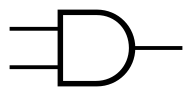
\includegraphics[scale=0.5]{pic/circuit_and.png}   %以pic.jpg的0.5倍大小输出
        \end{minipage}
    }
    \subfigure[逻辑或门] %第一张子图
    {
        \label{fig:or-gate}
        \begin{minipage}{4cm}
            \centering          %子图居中
            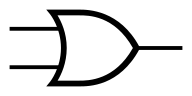
\includegraphics[scale=0.5]{pic/circuit_or.png}   %以pic.jpg的0.5倍大小输出
        \end{minipage}
    }
    \subfigure[逻辑非门] %第一张子图
    {
        \label{fig:not-gate}
        \begin{minipage}{4cm}
            \centering          %子图居中
            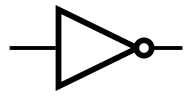
\includegraphics[scale=0.5]{pic/circuit_not.png}   %以pic.jpg的0.5倍大小输出
        \end{minipage}
    }

    \caption{与或非门(ANSI及IEEE标准)} %  %大图名称
    \label{fig:and-or-not-gate}  %图片引用标记
\end{figure}

而在量子电路中的计算则由一系列逻辑门、测量与赋值操作构成。但是,不同于传统电路是用金属线所连接以传递电压信号或电流信号;在量子线路中,线路是由时间所连接,亦即量子比特的状态随着时间自然演化,一直到遇上逻辑门而被操作。另一方面,经典计算机的大多数基本逻辑门(除了非门)都是不可逆的,例如,对于与门,我们不可能从输出信息的每一位恢复到两个输入信息;而量子计算中的每一步操作都是酉变换。刚刚的几个酉变换在量子电路中都有他们的电路元件表示

\begin{figure}[H]
    \centering
    \begin{minipage}{12cm}
        \centering\Qcircuit @C=1em @R=2em @!C @!R {
        \lstick{\hbox{$\ket{0}$}} & \gate{\hbox{$H$}} & \gate{\hbox{$Z$}} & \gate{\hbox{$X$}} & \gate{\hbox{$U_{-\frac{\pi}{4}}$}} & \meter & \cw \\
        }
    \end{minipage}
\end{figure}
上面的过程中,量子比特的变换过程为 \begin{align*}
    \begin{bmatrix} 0 \\1 \end{bmatrix}\to
    \frac{1}{\sqrt{2}}\begin{bmatrix} 1 \\1 \end{bmatrix}\to
    \frac{1}{\sqrt{2}}\begin{bmatrix} 1 \\-1 \end{bmatrix}\to
    \frac{1}{\sqrt{2}}\begin{bmatrix} -1 \\1 \end{bmatrix}\to
    \begin{bmatrix} 1 \\0 \end{bmatrix}\xrightarrow{\text{measure}}\ket{\psi}
\end{align*}

在实际的计算中,仅仅进行单元操作显然是不够的,因此需要考虑将对单量子比特的操作拓展到多量子比特, 从一种简单的情况出发。现在有两个量子比特,但是仅对其中的一个,即目标量子比特进行操作,另一个作为控制量子比特,决定是否对目标进行否运算, 于是容易得到这一操作的酉矩阵 \begin{align}\begin{aligned}
        U_{\text{CNOT}}=\begin{bmatrix}
                            1 & 0 & 0 & 0 \\
                            0 & 1 & 0 & 0 \\
                            0 & 0 & 0 & 1 \\
                            0 & 0 & 1 & 0
                        \end{bmatrix}
    \end{aligned}\end{align}
当且仅当控制量子比特为 $1$ 时, 目标量子比特通过非门. 可以被表示为 $\ket{A,B}\to\ket{A,B\xor A}$。因此也被形象地表示为
\begin{figure}[H]
    \label{fig:cnot-gate}
    \centering
    \subfigure{
        \begin{minipage}{6cm}
            \centering
            \Qcircuit @C=1em @R=2em @!C @!R {
            &\gate{CNOT} & \qw
            }
        \end{minipage}
    }=
    \subfigure {
        \begin{minipage}{6cm}
            \centering
            \Qcircuit @C=1em @R=2em @!C @!R {
            &\ctrl{1} & \qw\\
            &\targ & \qw
            }
        \end{minipage}
    }
    =
    \subfigure {
        \begin{minipage}{6cm}
            \centering
            \Qcircuit @C=1em @R=2em @!C @!R {
            &\ctrl{1} & \qw\\
            &\gate{X} & \qw
            }
        \end{minipage}
    }
\end{figure}

理论研究证明,任何多量子比特逻辑门可以由受控非门和单量子门组成\cite{nielsen2002quantum},因此,受控非门具有通用性,这也与经典电路中与非门(XAND)的通用性相对应。

下面介绍几个量子电路的简单应用。交换两个量子比特的电路可以被表示为

\begin{figure}[H]
    \centering
    \begin{minipage}{12cm}
        \centering
        \Qcircuit @C=1em @R=2em @!C @!R {
        &\ctrl{1}&\targ&\ctrl{1}&\qw\\
        &\targ&\ctrl{-1}&\targ\\
        }
    \end{minipage}
\end{figure}

这是因为容易验证 \begin{align}\begin{aligned}
        \ket{a,b} & \to\ket{a,a\xor b}                              \\
                  & \to\ket{a\xor(a\xor b),a\xor b}=\ket{b,a\xor b} \\
                  & \to\ket{b,(a\xor b)\xor b}=\ket{b,a}.
    \end{aligned}\end{align}

如果在二维 Hadamard 门后面跟着一个 CNOT 门
\begin{figure}[H]
    \centering
    \begin{minipage}{12cm}
        \centering
        \Qcircuit @C=1em @R=2em @!C @!R {
        \lstick{\hbox to 2em{$\ket{00}$\hss}} & \gate{\hbox{$H^{\tensor 2}$}} & \gate{\hbox{$CNOT$}} & \meter & \cw \\
        }
    \end{minipage}
\end{figure}
对四个二维本征态进行计算, 我们会得到 \begin{align}\begin{aligned}
        \ket{00}\mapsto\ket{\beta_{0,0}}\frac{\ket{00}+\ket{11}}{\sqrt{2}} \\
        \ket{01}\mapsto\ket{\beta_{0,1}}\frac{\ket{01}+\ket{10}}{\sqrt{2}} \\
        \ket{10}\mapsto\ket{\beta_{1,0}}\frac{\ket{00}-\ket{11}}{\sqrt{2}} \\
        \ket{11}\mapsto\ket{\beta_{1,1}}\frac{\ket{00}-\ket{10}}{\sqrt{2}}
    \end{aligned}\end{align}
概括地 \begin{align}\begin{aligned}
        \ket{\beta_{x,y}}=\frac{\ket{0,y}+(-1)^x\ket{1,\overline{y}}}{\sqrt{2}}.
    \end{aligned}\end{align}

这就是著名的 Bell 态(或 EPR\footnote{Einstein-Podolsky-Rosen} 对),它描述了一种最简单的量子纠缠示例:上面的四个量子比特虽然都具有两个维度,但是在测量中,只要测量了其中的一维,另一维也被唯一地确定了。Bell 态的这一性质使其在超密编码与量子隐形传态的领域扮演着重要的角色。

\subsection{量子电路的设计:Deutsch-Jozsa 算法\label{sec:deutsch}}

Desutsch-Jozsa 算法可由一个简单的游戏进行引入:Alice 从 $0-2^{n}-1$ 中选一个数 $x$ 并将其传送给 Bob。Bob 计算出某个函数 $f(x)$ 的值,可以为 $0$ 或 $1$,并将它传回给 Alice。已知该函数只有可能有两种情况:要么 $f(x)$ 对于所有的 $x$ 均为常数,要么 $f(x)$ 恰好对于一半的 $x$ 取 $0$,一半的取 $1$。Alice 怎样能够最快地判断 $f(x)$ 的类型?

形式化地,已知函数 $f:\{0,1\}^{\otimes n}\rightarrow\{0,1\}$ 一定是下列两种极端形式的一种:
\begin{enumerate}
    \item Constant:$f(x)\equiv 0\text{ or }f(x)\equiv 1$;
    \item Balanced:$f(x)=0~~\text{for half of }\{0,1\}^{\otimes n},\text{ and }f(x)=1~~\text{for the other half}$
\end{enumerate}

问如何用最少的查询次数确定 $f$ 属于二者中的哪一种。

\begin{figure}[H]
    \centering
    \begin{minipage}{12cm}
        \centering
        \def\ingate{\vbox to 3.5em{\hbox to 4em{\tiny$x$\hss $x$}\vss
                    \hbox to 4em{\Large\hss$U_f$\hss}\vss
                    \hbox to 4em{\medmuskip1mu\tiny$x$\hss $y\oplus f(x)$}\vskip-2pt}}
        \Qcircuit @C=1em @R=2em {
        \lstick{\hbox to 2em{$\ket{0}^{\tensor n}$\hss}} & {/}\qw& \qw & \gate{\hbox{$H^{\otimes n}$}} & \multigate{1}{\ingate} & \gate{\hbox{$H^{\otimes n}$}} & \qw & \meter \\
        \lstick{\hbox to 2em{$\ket{0}$\hss}} & \qw & \gate{X} & \gate{H} & \ghost{\ingate} & \qw & \qw & \\
        }
    \end{minipage}
    \caption{Deustch-Jozsa 算法的量子电路}
    \label{fig:deu-joz}
\end{figure}

考虑图 \ref{fig:deu-joz} 所示量子电路,输入 $U_f$ 的初态为 $\ket{+}^{\tensor n}\ket{-}$。考虑初态的前 $n$ 位,设其在某一状态下为 $x$,那么 \begin{align}
    U_f\ket{x}\ket{-}=\ket{x}\ket{-\tensor f(x)}=(-1)^{f(x)}\ket{x}\ket{-}.
\end{align}
从而 \begin{align}
    U_f\ket{+}^{\tensor n}\ket{-}=\sum_{x\in\{0,1\}^{\tensor n}}\frac{(-1)^{f(x)}}{\sqrt{2^n}}\ket{x}\ket{-}.
\end{align}
另外,容易验证,对于单量子比特门 $H\ket{x}=\sum_{z\in\{0,1\}}(-1)^{xz}\ket{z}/\sqrt{2}$,将这一结果推广到 $n$ 个量子比特上,就有了 \begin{align}
    H^{\tensor n}\ket{x}=\sum_{z\in\{0,1\}^{\tensor n}}\frac{(-1)^{x\cdot z}}{\sqrt{2^n}}\ket{z}.
\end{align}
从而 \begin{align}
    H\left(\sum_{x\in\{0,1\}^{\tensor n}}\frac{(-1)^{f(x)}}{\sqrt{2^n}}\ket{x}\right)=\sum_{x,z\in\{0,1\}^{\tensor n}}\frac{(-1)^{x\cdot z+f(x)}}{2^n}\ket{z}\xrightarrow{\text{measure}}\ket{\psi}
\end{align}
于是考虑测量结果在 $\bra{0^{\tensor n}}$ 上的分量,即 $z$ 只取 $\ket{0}^{\tensor n}$ 时表达式的值 \begin{align}
    \inner{0^{\tensor n}}{\psi}=\sum_{x\in\{0,1\}^{\tensor n}}\frac{(-1)^{f(x)}}{2^n}
\end{align}
因此,当 $f$ 为常值函数时,测量结果必为 $\ket{0}^{\tensor n}$;当 $f$ 为平衡函数时,测量结果不可能出现 $\ket{0}^{\tensor n}$。在整个过程中,运用了 $3$ 个 $n$ 量子比特门,总时间复杂度在 $O(n) = O(\log N)$ 级别,相比于朴素算法 $O(N)$ 的时间开销,量子算法在效率上产生了质的飞跃。Deustch-Jozsa 算法是第一个具有重要意义的量子算法,其出现证明了量子计算在一些方面有着经典计算机无可比拟的性能,为接下来出现的许多量子算法奠基。
\section{量子算法应用:以 ACM 班程序设计作业为例}

\subsection{背景与题目}

在量子算法发明之初,以 Deutsch-Jozsa 为例的多种算法应用范围都相对局限,对于多数实际问题都无能为力或无法带来显著变化。但随着量子算法的逐步发展,许多经典计算机能解决的问题都能被量子计算机找到更优的方案。下面以上海交通大学 ACM 班 2022 级程序设计大作业的一道题\,\href{https://acm.sjtu.edu.cn/OnlineJudge/problem?problem_id=1754}{P1754 int2048-乘法速度测试} 为例,讲解量子算法的简单应用。

\subsection{前置知识}

在离散傅里叶变换(Discrete Fourier Transform,DFT)中,我们熟知求多项式 $f(x)$ 进行点值 $(\omega_N^k,y_k)$ 求值的方法 \begin{align*}
    y_k=\frac{1}{\sqrt{N}}\sum_{j=0}^{N-1}x_j\omega_N^{jk}.
\end{align*}
在经典计算机中,可以通过分治加速的方式将这一过程(快速傅里叶变换,Fast Fourier Transform)的时间复杂度优化为 $O(n\log n)$\cite{cooley1965algorithm}。在量子计算机中,我们同样希望进行相同的变换,使得 $N-1$ 维量子态 $\ket{X}=\sum_{j=0}^{N-1}x_j\ket{j}$,经过变换得到 $\ket{Y}=\sum_{k=0}^{N-1}y_k\ket{k}$,其中 $y_k$ 与 $x_k$ 的关系满足上式,$\ket{j},\ket{k}$ 表示其二进制分解所得结果的张量积。代入可得 \begin{align*}
    \ket{Y}=\sum_{k=0}^{N-1}y_k\ket{k}=\sum_{k=0}^{N-1}\left(\frac{1}{\sqrt{N}}\sum_{j=0}^{N-1}x_j\omega_N^{jk}\ket{k}\right)=\sum_{j=0}^{N-1}x_j\left(\frac{1}{\sqrt{N}}\sum_{k=0}^{N-1}\omega_N^{jk}\ket{k}\right)
\end{align*}
对比 $\ket{X},\ket{Y}$ 的形式,发现变换的实质就是一次基变换 \begin{align}\begin{aligned}
        \ket{j}\to\frac{1}{\sqrt{N}}\sum_{k=0}^{N-1}w_N^{jk}\ket{k}\label{eq:qft-change-basis}
    \end{aligned}\end{align}
两组标准正交基的变换可改写为酉变换 \begin{align*}
    U_{\text{QFT}} = \frac{1}{\sqrt{N}}
    \begin{bmatrix}
        1      & 1               & 1                         & \cdots & 1                      \\
        1      & \omega_N        & \omega_N ^{2}             & \cdots & \omega_N ^{N-1}        \\
        1      & \omega_N ^{2}   & \omega_N ^{4}             & \cdots & \omega_N ^{2(N-1)}     \\
        1      & \omega_N ^{3}   & \omega_N ^{6}             & \cdots & \omega_N ^{3(N-1)}     \\
        \vdots & \vdots          & \vdots                    & \ddots & \vdots                 \\
        1      & \omega_N ^{N-1} & \omega_N ^{(N-1)\times 2} & \cdots & \omega_N ^{(N-1)(N-1)}
    \end{bmatrix}
\end{align*}
这样就完成了一个满足量子计算要求的傅里叶变换算法,也即量子傅里叶变换(Quantum Fourier Transform,QFT)。

\subsection{电路设计}

上面的内容已经完成了量子傅里叶变换的算法设计,但得到了这样的酉阵,还不能直接设计出所需的量子电路,因此,在这里将式 \ref{eq:qft-change-basis} 进行进一步演化:考虑直接对 $\omega_{2^n}^{jk}=\exp(\frac{2\pi\mathrm{i} jk}{2^n})$ 指数中的 $\frac{k}{2^n}$ 进行二进制小数分解,也即对 $k$ 进行二进制分解,得到 \begin{align}\begin{aligned}
        \ket{j}\to\frac{1}{\sqrt{N}}\sum_{k=0}^{N-1}w_N^{jk}\ket{k}
         & =2^{-\frac{n}{2}}\sum_{l\in[n],k_l\in\{0,1\}}\exp\left(2\pi\mathrm{i} j\sum_{l\in[n]}k_l2^{-l}\right)\ket{k_1,\cdots,k_n}                  \\
         & =2^{-\frac{n}{2}}\bigotimes_{l\in[n]}\left(\sum_{k_l\in[0,1]}\exp(2\pi\mathrm{i} jk_l2^{-l})\ket{k_l}\right)                               \\
         & =2^{-\frac{n}{2}}\bigotimes_{l\in[n]}\left(\ket{0}+\exp(2\pi\mathrm{i} j2^{-l})\ket{1}\right)                                              \\
         & =2^{-\frac{n}{2}}\bigotimes_{l\in[n]}\left(\ket{0}+\exp\left(2\pi\mathrm{i}\left\{\frac{j}{2^l}\right\}\right)\ket{1}\right)\label{eq:qft}
    \end{aligned}\end{align}
这里的 $\{\frac{j}{2^l}\}$ 表示取 $\frac{j}{2^l}$ 的小数部分,由于 $e^{2\pi\mathrm{i}}=1$,因此等式是成立的。为了方便构建电路,记 \begin{align*}
    \frac{j}{2^n}=\overline{0.j_1 j_2\cdots j_n}
\end{align*}
那么式 \ref{eq:qft} 就可以写作 \begin{align*}
    2^{-\frac{n}{2}}\bigotimes_{l\in[n]}\left(\ket{0}+\exp(2\pi\mathrm{i}\overline{0.j_{n-l+1}\cdots j_{n}})\ket{1}\right)
\end{align*}
这种张量积意义下的量子电路就可以直接通过旋转门 $R_k$ 生成,\begin{align*}
    R_k=\begin{bmatrix}
            1 & 0                                           \\
            0 & \exp\left(\frac{2\pi\mathrm{i}}{2^k}\right)
        \end{bmatrix}
\end{align*}
例如,考虑输入态 $\ket{j_1,\cdots,j_n}$,由于 $\ket{0}=\ket{+},\ket{1}=\ket{-}$,将其首位通过 $H$ 门将得到 \begin{align*}
    \frac{1}{\sqrt{2}}\left(\ket{0}+\exp(2\pi\mathrm{i}\overline{0.j_1})\ket{1}\right)\ket{j_2,\cdots,j_n}
\end{align*}
随后,每次让首位通过受 $j_k$ 控的 $R_k$ 门,相位都将增加 $\frac{k\pi}{2^{k-1}}$,最终显然会得到 \begin{align*}
    \frac{1}{\sqrt{2}}\left(\ket{0}+\exp(2\pi\mathrm{i}\overline{0.j_1\cdots j_n})\ket{1}\right)\ket{j_2,\cdots,j_n}
\end{align*}
依此类推,每一位需要的状态都可以这样进行制备,这样就得到了量子电路\footnote{引用了 Michael Charemza 的 \LaTeX 代码 \cite{charemza2006examples}。}
\begin{figure}[H]
    \centering
    \begin{minipage}{12cm}
        \centering
        \Qcircuit @C=1em @R=2em {
        % \begin{bmatrix}
            \lstick{\ket{j_{n}}}   & \gate{H} & \gate{\hbox{$R_2$}} & \gate{\hbox{$R_3$}} & \qw    & \gate{\hbox{$R_n$}} & \qw      & \qw                 & \qw    & \qw                 & \qw      & \qw                 & \qw    & \qw                 & \qw      & \rstick{\ket{y_1}} \qw   \\
            \lstick{\ket{j_{n-1}}} & \qw      & \ctrl{-1}           & \qw                 & \qw    & \qw                 & \gate{H} & \gate{\hbox{$R_3$}} & \qw    & \gate{\hbox{$R_n$}} & \qw      & \qw                 & \qw    & \qw                 & \qw      & \rstick{\ket{y_2}} \qw   \\
            \lstick{\ket{j_{n-2}}} & \qw      & \qw                 & \ctrl{-2}           & \qw    & \qw                 & \qw      & \ctrl{-1}           & \qw    & \qw                 & \gate{H} & \gate{\hbox{$R_4$}} & \qw    & \gate{\hbox{$R_n$}} & \qw      & \rstick{\ket{y_3}} \qw   \\
            \lstick{\vdots }       &          &                     &                     & \ddots &                     &          &                     & \ddots &                     &          &                     & \ddots &                     &          & \rstick{\vdots }         \\
            \lstick{\ket{j_{1}}}   & \qw      & \qw                 & \qw                 & \qw    & \ctrl{-4}           & \qw      & \qw                 & \qw    & \ctrl{-3}           & \qw      & \ctrl{-2}           & \qw    & \ctrl{-2}           & \gate{H} & \rstick{\ket{y_{n}}} \qw
        % \end{bmatrix}
        }
    \end{minipage}
    \label{fig:qft-circuit}
\end{figure}

\section{思考与展望}

在过去的一段时间里,我对量子计算这一领域进行了初步的了解与学习。从一开始,对量子的叠加性特点与对量子比特进行数学计算方法的困惑,后来,通过检索资料、求助同学等方式,我逐渐理解了量子计算的原理,并通过与经典计算机的对比理解了量子计算的诸多特点;下面简要概括我对此的一些思考。

在深入学习之前,我一直不理解的一个问题是:如果说量子计算可以直接由矩阵与向量等传统数学操作完成,那么它和经典计算机中直接进行数学运算的区别在哪里?为什么可以带来效率的提升?后来,通过学习节 \ref{sec:deutsch} 中用 Deustch-Jozsa 算法,我形成了较为直观的理解:考虑一个 $n$ 量子比特门,对于一个酉变换,它能在 $O(n)$ 的时间内完成量子比特的变换,表面上看仅仅是改变了 $n$ 个比特位上的概率分布,实际上却同时改变了关于一组 $2^n$ 个标准正交基的线性组合。这就意味着,如果初态与变换选取得当,量子计算就可以用 $O(n)$ 的时间完成 $O(2^n)$ 的工作。这样的案例,也即刚刚提到的 Deustch-Jozsa 算法,已经在前文中展示了。

在了解了简单的几种量子算法后,我产生了进一步的好奇:目前有哪些类型的量子算法,它们能解决哪些经典计算机科学中的问题?\textit{ Quantum Computation and Quantum Information}\cite{nielsen2002quantum} 中对现有的量子算法进行了这样的分类:基于傅里叶变换的量子算法,例如 Shor 的素因子分解和离散对数算法;量子搜索算法,例如大名鼎鼎的 Grover 搜索;以及量子模拟算法。此前一段时间里我主要学习的是第一类量子算法。在尝试学习后面两种算法时,遇到的瓶颈在于对复向量空间的变换还没有建立起一个很好的几何直观,因此对例如 Grover 搜索中的 Amplitude Amplification 与迭代操作并没有理解得很透彻,希望在本学期结束后继续这一领域的学习。

展望量子计算领域的未来发展,这一结合物理原理、数学知识与计算机科学思想的计算方法,能带来跨时代意义的进步,具有相当光明的前景。不过在工程领域中,业界许多人认为该领域的前景具有很强的不确定性;很大程度上这是因为量子计算机的物理实现进展较为缓慢,理论领域的许多算法在工程上依旧无法进行实现。为了实现量子计算机,人们也提出了多种方案,目前较为热门的有超导量子计算、量子点量子计算等。回到理论领域,尽管现在已经有许多高效的量子算法,但它们的应用范围还是相对狭窄,学者们一直在致力于拓展量子算法的应用范围,并降低其不确定性;目前,对于很多量子计算相关问题的研究还非常有限\cite{孙晓明2016量子计算若干前沿问题综述},例如量子计算机多项式时间能否解决经典计算机在多项式时间所不能求解的问题, 即 BQP 是否等于 BPP。希望在不远的未来,量子计算领域的相关工作能取得进一步进展,人们对于量子计算能力的认识能变得更加全面。


\bibliographystyle{unsrt}
\bibliography{reference}

\end{document}